\newpage
\section{Abstract}

Diese Dokumentation beschreibt die Entwicklung eines autonomen Fahrzeuges im Projektmodul Pren 1 an der Hochschule Luzern. Das Fahrzeug soll Hindernisse bewältigen und flexibel auf Änderungen in einem vorgegebenen Wegenetz reagieren können. Das Ziel ist die Entwicklung eines Konzepts, das durch technische Innovation und Nachhaltigkeit überzeugt. Gleichzeitig soll es möglichst robust und einfach aufgebaut sein.
Das Vorgehen umfasst die Erstellung einer umfassenden Anforderungsliste, die Konzeption und Umsetzung eines Simulators, die Auswahl geeigneter Technologien aufgrund einer fundierten Technologierecherche und schliesslich die Ausarbeitung eines Lösungskonzeptes. Für letzteres wird zu einigen Funktionen Nutzwertanalysen und schliesslich ein Morphologischer Kasten, mit zwei Lösungsansätzen erstellt und ausgewertet. Durchsetzen kann sich das Prinzip Roomba (siehe Abbildung \ref{img:Visualisierung Fahrzeug}). Alle Antriebe werden der Einfachheit halber und aufgrund ihres geringen Gewichtes mit DC-Motoren realisiert. Um die Hindernisbewältigung möglichst simpel zu halten, kommt sie mit einem einzelnen Antrieb aus. Ein Simulator erlaubt die einfache Entwicklung und Überprüfung der Programmlogik, die für die Wegfindung verwendet wird. Mit Hilfe eines separaten Digital Twin können zudem digitale Tests durchgeführt, sowie weitere Daten erhoben werden, ohne einen physischen Prototypen zu benötigen. 
Im nächsten Semester im Modul Pren 2 wird das Konzept anhand eines physischen Prototyps umgesetzt und getestet. Als Abschluss findet ein Wettbewerb gegen die übrigen Teams statt, dabei muss die Funktionalität unter Beweis gestellt werden.

\begin{figure}[H] % 'h' steht für here, was bedeutet, dass das Bild möglichst an dieser Stelle eingefügt wird
    \centering
        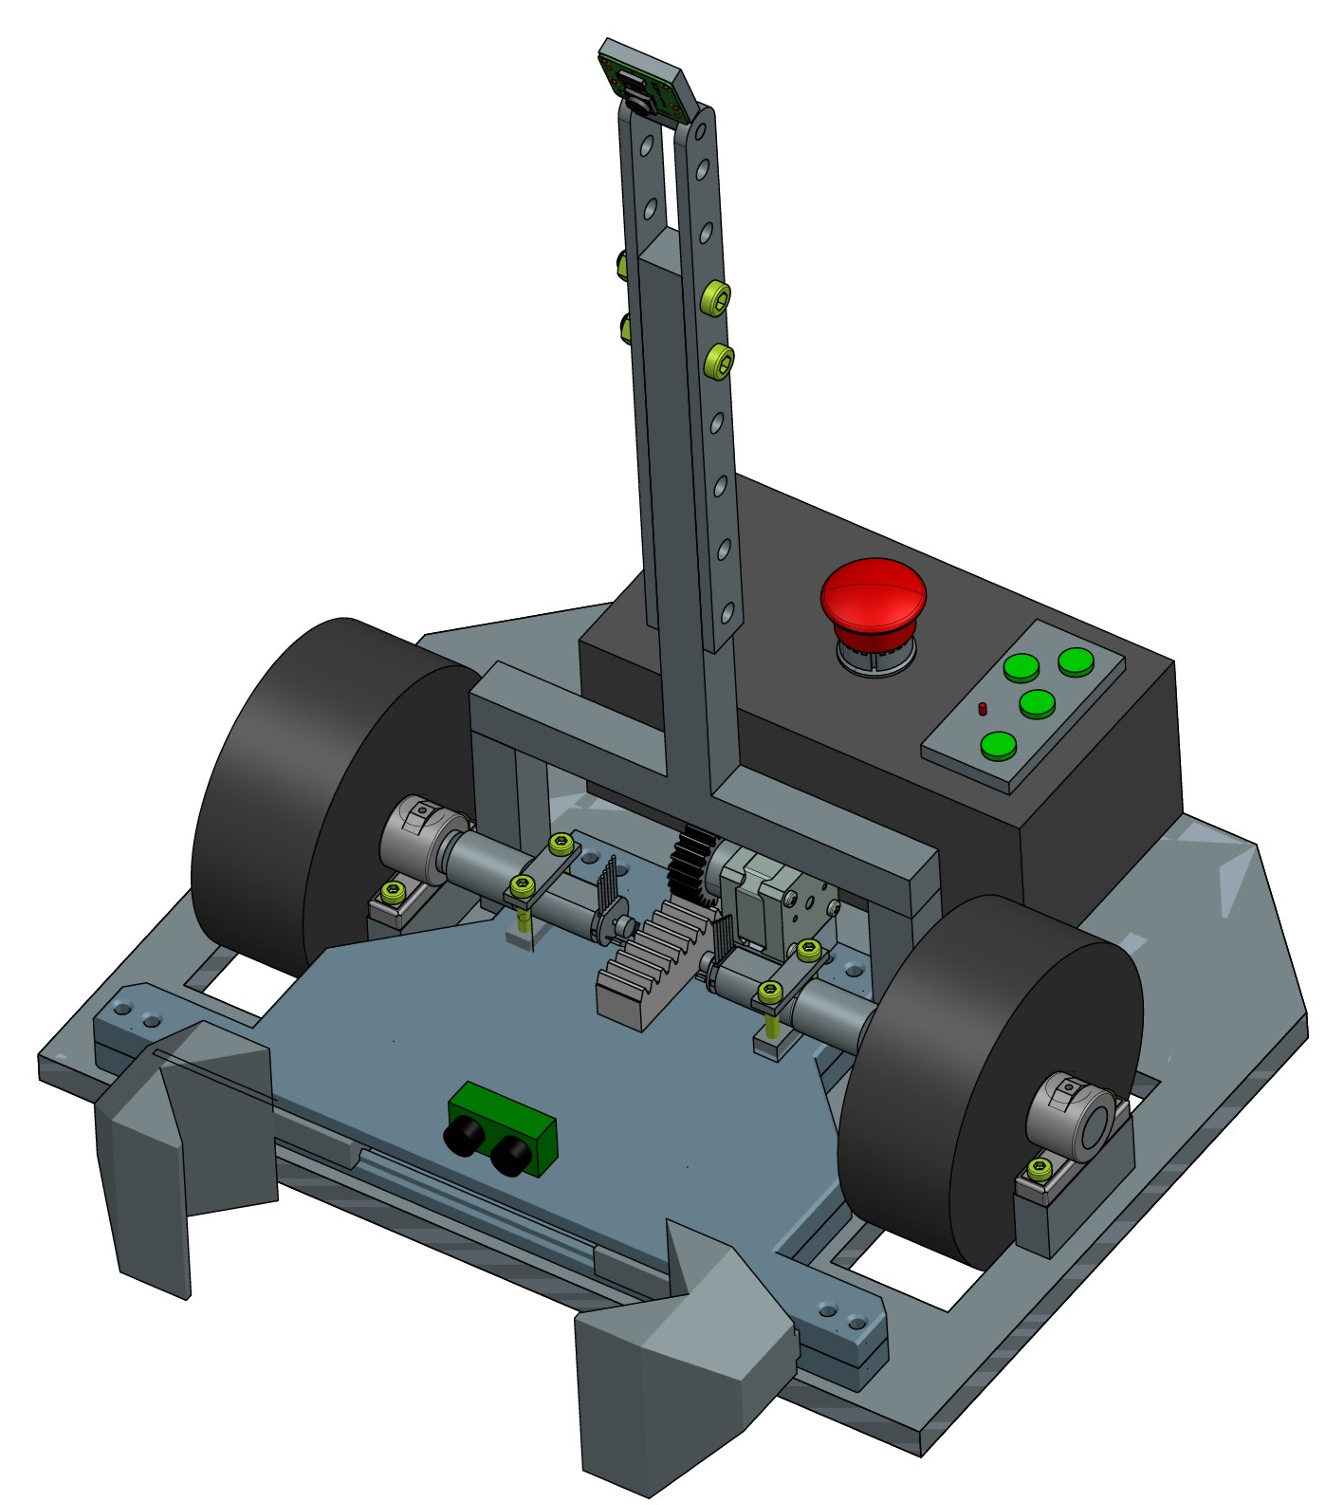
\includegraphics[width=0.5\linewidth]       {Skizze_Fahrzeug.png}               \caption[Visualisierung Fahrzeug]
        {Visualisierung Fahrzeug}
        
        \label{img:Visualisierung Fahrzeug}
    \end{figure} 